\documentclass[aspectratio=169,usenames,dvipsnames]{beamer}
\usepackage{preamble}
\title{Coding for Humanities, week 5}

\begin{document}

\begin{frame}
 \titlepage
\end{frame}

\begin{frame}{Last week}
    Files \& directories

    \vspace{1em}
    Libraries

    \vspace{1em}
    Midterm
\end{frame}

\begin{frame}{Plan for today}
 \tableofcontents
\end{frame}

\section{The Midterm}

\begin{frame}
    \begin{reference}
        \scriptsize\vspace{1em}
        \hfill Source: \url{https://oktop.tumblr.com/post/15352780846}
    \end{reference}
    \begin{columns}[b]
        \column{0.5\linewidth}
            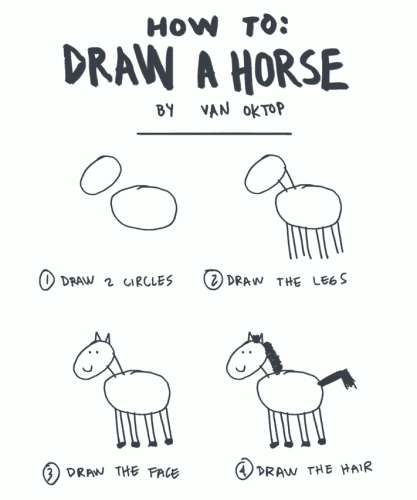
\includegraphics[height=0.9\textheight]{fig/horse1}
        \pause
        \column{0.5\linewidth}
            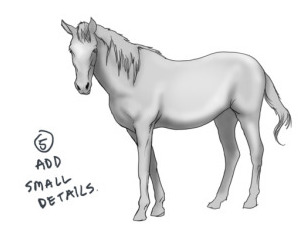
\includegraphics[width=0.9\linewidth]{fig/horse2}
    \end{columns}
\end{frame}

\begin{frame}{The Midterm}
    \begin{itemize}
        \item Solutions on Brightspace.
        \item Grades include \structure{feedback}
        \item Questions? Ask during the lab
    \end{itemize}
\end{frame}

\begin{frame}[fragile]{Common mistakes}
    \begin{itemize}
        \item Learn how to create functions
        \item Use \lstinline{return}, not \lstinline{print} at the end of a function
        \item All code should be inside the function; e.g., \lstinline{words = text.split()}
        \item In a for loop, results should accumulate; repeating a normal assignment \lstinline{a = ...} is not helpful
        \item Logic errors: If a character is not a vowel, it's not necessarily a consonant (could be punctuation)
        \item Know the methods of objects; e.g., cannot \lstinline{append()} to a dictionary

        \item Instead of repeating code, assign it to a variable \\
            e.g., \lstinline{words = text.split()}
        %\item Remember that you can use a function defined before \\
        %    to make your code simpler
        %\item Do not use the same variable name twice\\
        %    e.g., \lstinline{freq} parameter, and \lstinline{freq} dictionary
        %\item Split text into lines and words when needed
        %\item \lstinline{return} usually goes after a \lstinline{for} loop (not inside)
        %\item No \lstinline{return} at end of function
        %\item Returning a string of digits instead of list of numbers \\
        %    \lstinline{'123456...'} vs \lstinline{[123, 456, ...]}
        %\item Forgetting to \structure{call} a method:
        %    \lstinline{message = message.upper} \\
        %    \lstinline{for a, b in table.items}
    \end{itemize}

    \vspace{1em} Read the instructions carefully!
\end{frame}

\section{Improving code}
\subsection{Working code}
\frame{\tableofcontents[currentsection]}
\begin{frame}{Working code}
    \begin{definition}
        \structure{Debugging}: identify and fix errors (`bugs') in programs
    \end{definition}

    \pause\vspace{1em}
    \begin{columns}
        \column{0.5\linewidth}
            ``If debugging is the art of removing bugs from programs,
            programming must be the art of inserting them''
            (attributed to Edsger Dijkstra)

            % If you want more effective programmers, you will discover that they should not waste their time debugging, they should not introduce the bugs to start with.
            % (Edsger Dijkstra)
        \column{0.5\linewidth}
            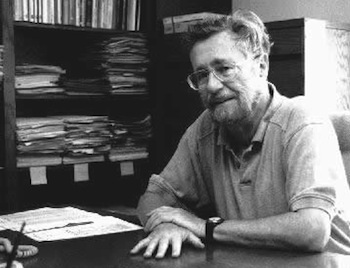
\includegraphics[height=0.5\textheight]{fig/dijkstra}

            \vspace{1em}
            Interview: \url{https://youtu.be/mLEOZO1GwVc}
    \end{columns}
\end{frame}

\begin{frame}{Intermezzo: actual bugs \dots}
    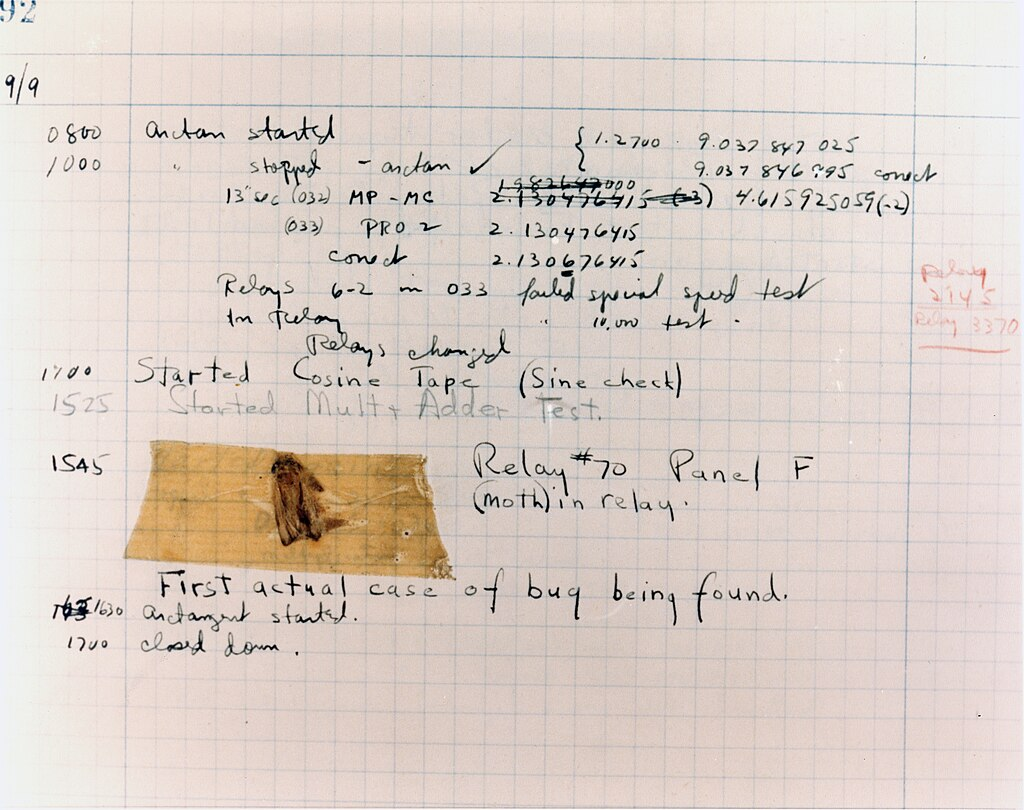
\includegraphics[height=0.8\textheight]{fig/bug}

    Source: U.S. Naval Historical Center Online Library Photograph NH 96566-KN
\end{frame}



\begin{frame}{More quotes}
    \begin{columns}
        \column{0.8\linewidth}
    \begin{quote}\normalfont
    On two occasions I have been asked, ---"Pray, Mr. Babbage, if you put
    into the machine wrong figures, will the right answers come out?"

	%In one case a member of the Upper, and in the other a member of the Lower
	% House put this question.
    [\dots]

    I am not able rightly to apprehend the kind of
	confusion of ideas that could provoke such a question.
	
    \end{quote}
        \column{0.2\linewidth}
    \end{columns}
	\vspace{1em}
    Charles Babbage, Passages from the Life of a Philosopher (1864), ch. 5:
    "Difference Engine No. 1"
\end{frame}

%\begin{frame}{More quotes}
%    \begin{quote}\normalfont
%    And programming computers was so fascinating.
%
%	You create your own little universe,
%
%	and then it does what you tell it to do.
%    \end{quote}
%
%	\vspace{1em}
%    Vint Cerf, a "father of the internet," quoted in "Your Life: Vinton Cerf"
%    interview with David Frank in AARP Bulletin (December 2016, Vol. 57, No.
%    10, p. 28.)
%\end{frame}

\begin{frame}{More quotes}
    \begin{quote}\normalfont
    The programmer, like the poet, works only slightly removed from pure
    thought-stuff. He builds his castles in the air, from air, creating by
    exertion of the imagination. Few media of creation are so flexible, so
    easy to polish and rework, so readily capable of realizing grand
    conceptual structures....
    Yet the program construct, unlike the poet's words, is real in the sense
    that it moves and works, producing visible outputs separate from the
    construct itself. [...] The magic of myth and legend has come true in our
    time. One types the correct incantation on a keyboard, and a display
    screen comes to life, showing things that never were nor could be.

	\vspace{1em}
    Fred Brooks (1975) The Mythical Man-Month: Essays on Software Engineering
    p.\ 7
    \end{quote}
\end{frame}

%\begin{frame}{More quotes}
%    \begin{columns}
%        \column{0.7\linewidth}
%``There are two ways of constructing a software design:
%
%One way is to make it so simple that there are obviously no deficiencies,
%
%and the other way is to make it so complicated that there are no obvious deficiencies.
%
%The first method is far more difficult.''
%
%--- C. A. R. Hoare 
%        \column{0.3\linewidth}
%    \end{columns}
%\end{frame}

%\begin{frame}{More quotes}
%    \begin{columns}
%        \column{0.7\linewidth}
%    ``Everyone knows that debugging is twice as hard as writing a program in
%    the first place.
%
%	So if you're as clever as you can be when you write it,
%    how will you ever debug it?'' (Brian Kernighan)
%        \column{0.3\linewidth}
%    \end{columns}
%\end{frame}

\begin{frame}{More quotes}
    \begin{columns}
        \column{0.7\linewidth}
    Maurice Wilkes discovers debugging in 1949:

    \vspace{1em}
    \begin{quote}\normalfont
    ``As soon as we started programming, we found to our surprise that it
    wasn't as easy to get programs right as we had thought. Debugging had to be
    discovered. I can remember the exact instant when I realized that a large
    part of my life from then on was going to be spent in finding mistakes in
    my own programs.''
    \end{quote}
        \column{0.3\linewidth}
    \end{columns}
\end{frame}

\begin{frame}{How to find bugs?}
	\begin{enumerate}
		\item Code doesn't work \dots error message
        \item Code doesn't do what it should \dots (print variables)
		\item Tests (sprinkle if-statements!)
		\item Automated tools (e.g., pylint)
	\end{enumerate}
\end{frame}

\begin{frame}{Common errors}
    \begin{description}[AttributeError]
        \item[SyntaxError] missing comma, colon, parenthesis etc.
        \item[NameError] variable/function name typo
        \item[IndexError] \texttt{seq[n] with n >= len(seq)}
        \item[KeyError] key not in dict
        \item[AttributeError] \texttt{obj.att}, but obj does not have att
        \item[TypeError] mixing up str/int/etc.
        \item[ValueError] generic error: right type, wrong value
        \item[FileNotFoundError] check filename / path
        \item[\dots] \dots
    \end{description}
\end{frame}

\begin{frame}[fragile]{Understanding tracebacks; example 1}
\begin{definition}
    \structure{Traceback}: the chain of function calls that led to an error.
\end{definition}
\begin{lstlisting}
>>> sent = "The quick brown fox jumped."
>>> words = sent.split()
>>> print(words.lower())
Traceback (most recent call last):
  File "<stdin>", line 1, in <module>
AttributeError: 'list' object has no attribute 'lower'
>>>
\end{lstlisting}

First step: \structure{locate} the root cause.
\end{frame}

\begin{frame}[fragile]{Understanding tracebacks; example 2}
\begin{definition}
    \structure{Traceback}: the chain of function calls that led to an error.
\end{definition}
\begin{lstlisting}
>>> from os.path import splitext
>>> splitext(['not', 'a', 'filename'])
Traceback (most recent call last):
  File "<stdin>", line 1, in <module>
  File "/usr/lib/python3.7/posixpath.py", line 122, in splitext
    p = os.fspath(p)
TypeError: expected str, bytes or os.PathLike object, not list
>>>
\end{lstlisting}

First step: \structure{locate} the root cause.
Typically somewhere in your own code \dots
\end{frame}


\begin{frame}{General strategy}
    The most effective debugging tool is still careful thought, coupled with
    judiciously placed print statements. (Brian Kernighan)
    
    \pause\vspace{1em}
    Go through each line of code \dots
    \begin{itemize}
        \item Think like the computer: \\
            what is happening? \\
            Is it what you intended?
        \item Ask yourself: what is the input and output? \\
            Confirm: print values
        \item Does the problem only occur with particular values? \\
            What is special about them?
        \item For difficult problems: rinse \& repeat \dots
    \end{itemize}
\end{frame}



\subsection{Good code}
\begin{frame}{Good code: Refactoring}
    Insight: can achieve the same end in many different ways

    \pause
    \begin{definition}
        \structure{Refactoring}: improving code (e.g., readability) \\
            while keeping the same functionality (i.e., behavior).
    \end{definition}

    % FIXME: already mentioned in previous lectures
    % concrete examples, or leave out.
    \begin{itemize}
        \item Clear variable/function names
        \item Separate steps/functions
        \item No unnecessary steps
        \item No repetition
        \item Use idioms
    \end{itemize}
\end{frame}

\begin{frame}[fragile]{Example: working code}
\begin{lstlisting}
def clean_tweets(filename):
    with open(filename, encoding='utf8') as infile:
        text = infile.read()
        cleaned_text = ''
        lower_text = text.lower()
        for char in lower_text:
            if char not in '!$%^&*()-+={}[]:;"\'|<>,.?/~`':
                cleaned_text += char
        cleaned_list = cleaned_text.split()
        return cleaned_list
\end{lstlisting}
\end{frame}

\begin{frame}[fragile]{Example: re-factored}
\begin{columns}
\column{0.6\linewidth}
\begin{lstlisting}[style=smaller]
def remove_punc(text):
    punctuation = '!$%^&*()-+={}[]:;"\'|<>,.?/~`'
    return ''.join(char for char in text
            if char not in punctuation)

def clean_tweets(filename):
    with open(filename, encoding='utf8') as infile:
        text = infile.read()
    cleaned_text = remove_punc(text.lower())
    tokens = cleaned_text.split()
    return tokens
\end{lstlisting}
\column{0.4\linewidth}
\begin{itemize}
\item Separate function for punctuation
\item More efficient punctuation elimination
\item Limit scope of \lstinline{with}
\item Renamed \lstinline{cleaned_list} \\
    to \lstinline{tokens}
\end{itemize}
\end{columns}
\end{frame}

\begin{frame}{Code style guides}
    \begin{reference}
        PEP-0008: coding conventions for Python code.
        \url{https://www.python.org/dev/peps/pep-0008/}
    \end{reference}

    For larger projects, follow a style guide; e.g.,
    \begin{itemize}
        \item Max.\ 1000 lines per file
        \item Max.\ 25 lines per function
        \item Avoid spaghetti \& lasagna code
        \item etc.
    \end{itemize}
    % FIXME: not really applicable to notebook code
   
    \vspace{1em}
    \structure{But}:
        ``A Foolish Consistency is the Hobgoblin of Little Minds'' \\
        (Ralph Waldo Emerson, Self-Reliance)
\end{frame}



\subsection{Fast code}
\begin{frame}[fragile]{Fast code: Example}
    \begin{columns}[T]
\column{0.4\linewidth}
\begin{lstlisting}[style=smaller]
def counter(words):
    counts = {}
    for word in words:
        if word not in counts:
            counts[word] = 0
        counts[word] += 1
    return counts
\end{lstlisting}
% OR:
% from collections import Counter
% return Counter(words)
\column{0.6\linewidth}
\begin{lstlisting}[style=smaller]
def count_in_list(word_to_count, words):
    number_of_hits = 0
    for word in words:
        if word == word_to_count:
            number_of_hits += 1
    return number_of_hits

def counter2(words):
    counts = {}
    unique_words = set(words)
    for word in unique_words:
        counts[word] = count_in_list(word, words)
\end{lstlisting}
% OR: counts[word] = words.count(word)
\end{columns}
\end{frame}


\begin{frame}{Levels to optimize}
    \begin{description}
        \item[Hardware] get faster machine, more memory, etc.
        \item[Code] improve `constant' factors \\
			(caching, compact representations etc.)
        \item[Algorithm] e.g., sorting by random shuffling will never be fast \dots \\
			(algorithmic complexity)
        \item[Problem] e.g., sorting is harder than searching \\
			(computational complexity)
    \end{description}

    \pause
    \begin{itemize}
        \item Avoid doing unnecessary things
        \item Avoid slow methods
        \item Lots of clever things \dots (rabbit hole)
    \end{itemize}
\end{frame}

\begin{frame}{Efficiency}
    \begin{reference}
        \url{https://www.xkcd.com/1445/}
    \end{reference}
    \centering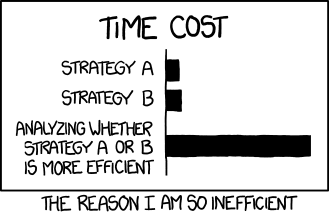
\includegraphics[height=0.6\textheight]{fig/xkcdefficiency}
\end{frame}


% \begin{frame}{Profiling}
%     \begin{definition}
%         \structure{Profiling}: identify performance bottlenecks by measuring
%     \end{definition}
%     
%     Two important measurements:
%     \begin{itemize}
%         \item How often is each function called
%         \item How long does it take?
%     \end{itemize}
% 
%     \pause\vspace{1em}
%     Consider two scenarios:
%     \begin{enumerate}
%         \item A 100x speedup of a component responsible for 1\% of total runtime.
%         \item A 1.1x speedup of a component responsible for 90\% of total runtime.
%     \end{enumerate}
%     Do not waste your time on 1; therefore: measure!
% \end{frame}
% 
% % \begin{frame}{Is it worth the time?}
% %     \begin{reference}\scriptsize\vspace{1em}
% %         \url{https://www.xkcd.com/1205/}
% %     \end{reference}
% %     \hfill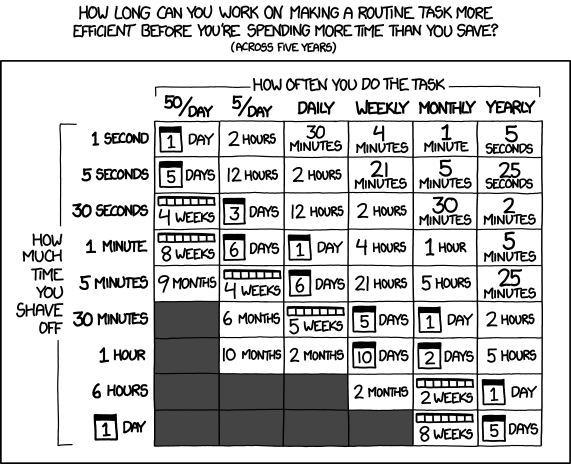
\includegraphics[height=0.9\textheight]{fig/xkcdworththetime}
% % \end{frame}
% 
% \begin{frame}{Takeaway}
%     ``We should forget about small efficiencies, say about 97\% of the time:
%     premature optimization is the root of all evil.
% 	\pause
% 	Yet we should not pass up our opportunities in the critical 3\%''
%     -- Donald Knuth
% 
%     \vspace{1em}
%     \begin{itemize}
%         \item Consider expected return on investment
%         \item Optimization risks overcomplicating \& over-engineering
%     \end{itemize}
% \end{frame}

\begin{frame}{Summary}
    Improving code involves
    \begin{itemize}
        \item Debugging
        \item Re-factoring, code style
        \item Optimization, profiling
    \end{itemize}
\end{frame}



% break


\section{Sentiment analysis}
\subsection{Identifying positive and negative language}
\frame{\tableofcontents[currentsection]}

\begin{frame}{Sentiment analysis}
    \begin{definition}
        \structure{Sentiment (polarity) analysis}: 
            is a piece of language positive or negative?
    \end{definition}

    Applications:
    \begin{itemize}
        \item Identify positive/negative reviews
        \item Monitor complaints about a company on social media
    \end{itemize}

    \pause
    How to estimate?
    \begin{itemize}
        \item Create sentiment word lists
        \item Assign each word a score, e.g.: \\
            negative vs positive, 5-point scale, etc.
        \item Positive: good, swell, benevolent, admire, etc. \\
                Negative: bad, sour, abnormal, hinder, etc.
        \item Combine scores for each word into a total score. \\
                (simple sum, or train classification model)
    \end{itemize}
\end{frame}

\begin{frame}{Challenges}
    Can we really reduce sentiment to counts of positive/negative words?

    \begin{itemize}
        \item Negation
        \item Polysemy
        \item Non-literal meaning
        \item etc. etc.
    \end{itemize}

	\vspace{1em}
    Still, the `stupid' model works surprisingly well.

    Many tricks for minor improvements.
\end{frame}

\begin{frame}[fragile]{Sentiment word counting in Python}
    \begin{reference}\scriptsize
        Word lists: \url{https://www.kaggle.com/rtatman/sentiment-lexicons-for-81-languages} \\
        Proper sentiment analysis: \url{https://www.twilio.com/blog/2017/12/sentiment-analysis-scikit-learn.html}
        % \https://stackabuse.com/python-for-nlp-sentiment-analysis-with-scikit-learn/}
        %\url{https://towardsdatascience.com/basic-binary-sentiment-analysis-using-nltk-c94ba17ae386}
        % Issues: uses NLTK's classifiers / API.
        % \url{https://nealcaren.org/lessons/wordlists/}
        % Issues: uses Pandas, relies on installing package w/sentiment lexicon;
        % no classifier
        %\url{http://www.nltk.org/howto/sentiment.html}
        % issues: NLTK classifiers, no explanation
    \end{reference}
\begin{lstlisting}[style=smaller]
import nltk
with open('data/sentiment/positive.txt', encoding='utf8') as inp:
    positive_words = set(inp.read().splitlines())
with open('data/sentiment/negative.txt', encoding='utf8') as inp:
    negative_words = set(inp.read().splitlines())
with open('VERNE Journey to Center of Earth.txt', encoding='utf8') as inp:
    words = nltk.word_tokenize(inp.read().lower())
\end{lstlisting}
\pause\vspace{-1em}
\begin{lstlisting}[style=smaller]
sentiment = 0
for word in words:
    if word in positive_words:
        sentiment += 1
    elif word in negative_words:
        sentiment -= 1
\end{lstlisting}
\end{frame}

\subsection{Does every story reduce to six basic plot shapes?}
% Show other/simpler example applications in literature?
\begin{frame}{Kurt Vonnegut: The simple shapes of stories}
    \begin{reference}
        More information:
        \url{https://www.brainpickings.org/2012/11/26/kurt-vonnegut-on-the-shapes-of-stories/}
    \end{reference}
    \begin{columns}
        \column{0.5\linewidth}
    \centering\large
    \url{https://youtu.be/oP3c1h8v2ZQ?t=20}
        \column{0.5\linewidth}\centering
        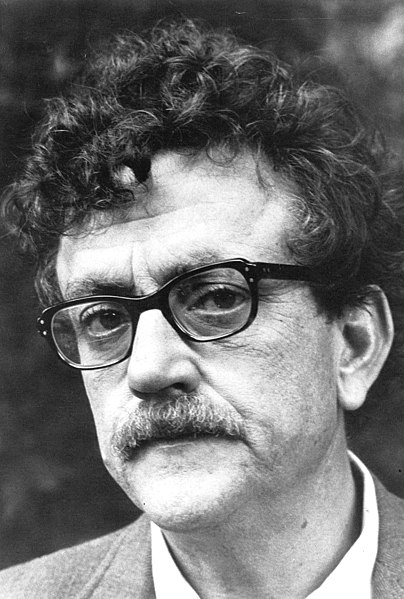
\includegraphics[height=0.5\textheight]{fig/vonnegut}
    \end{columns}
\end{frame}

\begin{frame}{Can we operationalize this?}
    \begin{reference}
        Matthew Jockers (2015) \url{http://www.matthewjockers.net/2015/02/02/syuzhet/} \\
        Reagan et al (2015) \url{https://doi.org/10.1140/epjds/s13688-016-0093-1}
    \end{reference}
    Yes we can!
    
    \begin{columns}
        \column{0.5\linewidth}
    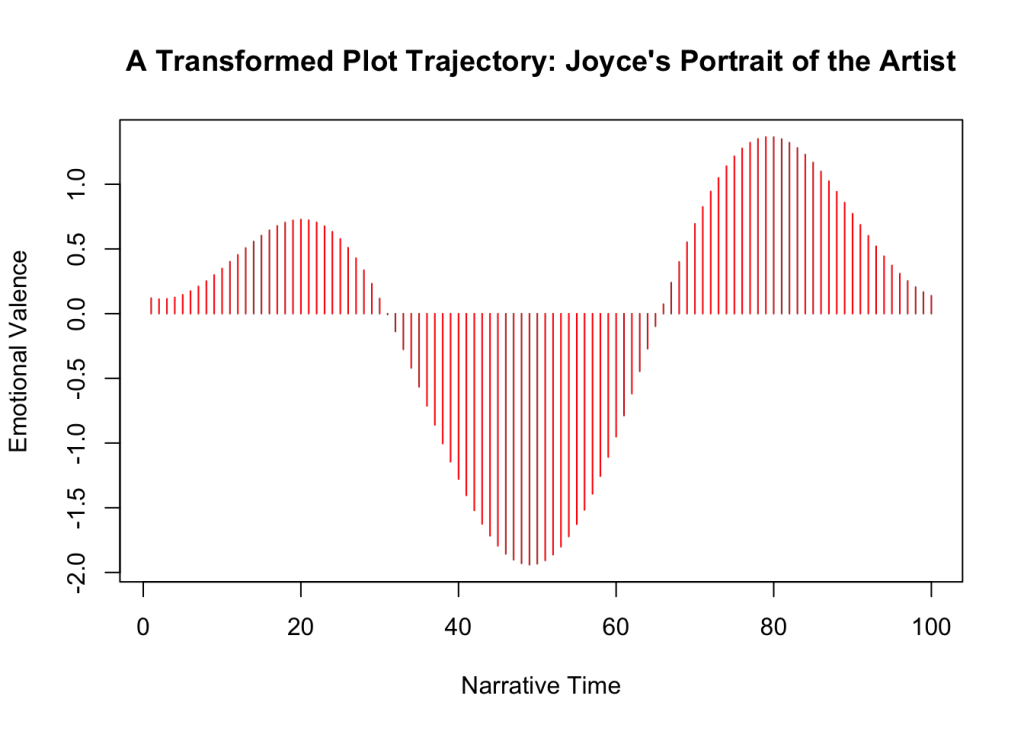
\includegraphics[width=1\textwidth]{fig/joycearc}

        \column{0.5\linewidth}
    \begin{itemize}
        \item Estimate emotions: count sentiment words
        \item Chop text into chunks of x words, count sentiment in each chunk
        \item Recognize plot shapes: SVD / Fourier transform
    \end{itemize}
    \end{columns}
    Seems to confirm that all novels have a few basic story shapes!
\end{frame}

\begin{frame}{But \dots Hold your horses!}
    \begin{reference}
        \url{https://annieswafford.wordpress.com/2015/03/07/continuingsyuzhet/} \\
        \url{https://senderle.github.io/svd-noise/}
    \end{reference}

    \begin{columns}
        \column{0.5\linewidth}
            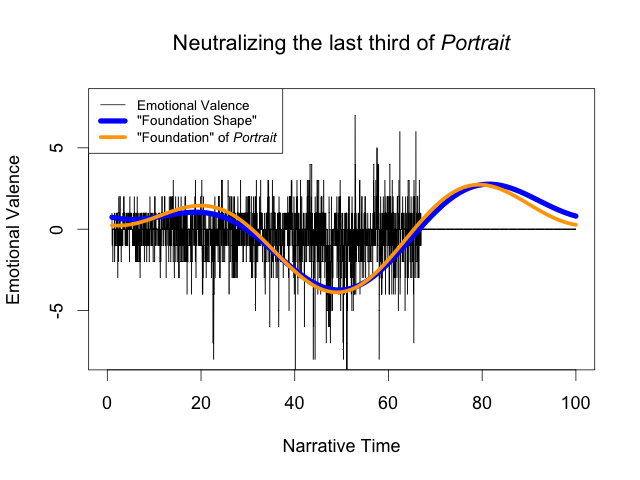
\includegraphics[width=0.9\linewidth]{fig/joycenoise}
        \column{0.5\linewidth}
    \begin{itemize}
        \item Reducing \structure{emotions} to binary sentiment word frequencies \\
            is naive \& crude
        \item The reduction to basic story shapes appears to be \\
            a reflection of noise and artefacts.
    \end{itemize}
    \end{columns}

    \pause
    Takeaway:
    \begin{itemize}
        \item Yes, if you insist, you can reduce anything to 6 story shapes \\
            (or 3, 10, 100, etc.)
        \item No, these shapes are probably not fundamental or universal
    \end{itemize}
\end{frame}

\begin{frame}{Summary}
    \begin{itemize}
        \item Sentiment in text can be measured
        \item Interesting patterns may emerge; but caveat emptor
    \end{itemize}
\end{frame}



\section{Keyword analysis}
\subsection{Keywords in context with NLTK}
\frame{\tableofcontents[currentsection]}

\begin{frame}[fragile]{NLTK: explore keywords in context}
    \begin{reference}
        \url{https://www.nltk.org/book/ch01.html}
    \end{reference}
    NLTK \texttt{Text} object offers:
    \begin{itemize}
        \item Concordance
        \item Similar words
        \item Common contexts
        \item Collocations
        \item Dispersion plot
    \end{itemize}
Make \texttt{Text} objects:
\begin{lstlisting}
In: import nltk
In: with open('MELVILLE Moby Dick.txt', encoding='utf8') as inp:
...     moby_dick = nltk.Text(nltk.word_tokenize(inp.read()))
In: with open('AUSTEN Sense and Sensibility.txt', encoding='utf8') as inp:
...     austen_sense = nltk.Text(nltk.word_tokenize(inp.read()))
\end{lstlisting}
\end{frame}

\begin{frame}[fragile]{Concordance}
\begin{lstlisting}
In: moby_dick.concordance('monstrous')
\end{lstlisting}
\begin{lstlisting}[style=plainsmaller]
Ho ' s Story . CHAPTER 55 . Of the Monstrous Pictures of Whales . CHAPTER 56 .
ong the former , one was of a most monstrous size ... . This came towards us ,
n of the Psalms_ . " Touching that monstrous bulk of the whale or ork we have r
ll over with a heathenish array of monstrous clubs and spears . Some were thick
d as you gazed , and wondered what monstrous cannibal and savage could ever hav
that has survived the flood ; most monstrous and most mountainous ! That Himmal
they might scout at Moby Dick as a monstrous fable , or still worse and more de
of Radney. ' " CHAPTER 55 . Of the Monstrous Pictures of Whales . I shall ere l
ing Scenes . In connexion with the monstrous pictures of whales , I am strongly
ere to enter upon those still more monstrous stories of them which are to be fo
ght have been rummaged out of this monstrous cabinet there is no telling . But
e of Whale-Bones ; for Whales of a monstrous size are oftentimes cast up dead u
\end{lstlisting}
\end{frame}

\begin{frame}[fragile]{Similar words}
\begin{reference}
Phillips (1969). Jane Austen's English. \url{https://www.jstor.org/stable/43342482}
\end{reference}
\begin{lstlisting}
In: moby_dick.similar("monstrous")
\end{lstlisting}
\begin{lstlisting}[style=plain]
mean part maddens doleful gamesome subtly uncommon careful untoward
exasperate loving passing mouldy christian few true mystifying
imperial modifies contemptible
\end{lstlisting}
\begin{lstlisting}
In: austen_sense.similar("monstrous")
\end{lstlisting}
\begin{lstlisting}[style=plain]
very heartily so exceedingly remarkably as vast a great amazingly
extremely good sweet
\end{lstlisting}

\structure{Insight}: monstrous is positive for Austen! \\
Austen uses monstrous as an adverb of degree (Phillips 1969, p.\ 329)
\end{frame}

\begin{frame}[fragile]{Common contexts}
\begin{lstlisting}[style=smaller]
In [6]: austen_sense.common_contexts(['monstrous', 'very'])
\end{lstlisting}
\begin{lstlisting}[style=plainsmaller]
a_pretty am_glad a_lucky is_pretty, be_glad
\end{lstlisting}

\pause\vspace{1em}
i.e., Sense \& Sensibility contains both ``a very pretty" \\
    and ``a monstrous pretty" etc.

\begin{lstlisting}
In: austen_sense.concordance('monstrous')
\end{lstlisting}
\begin{lstlisting}[style=plainsmaller]
Displaying 11 of 11 matches:
 `` Now , Palmer , you shall see a monstrous pretty girl . '' He immediately we
your sister is to marry him . I am monstrous glad of it , for then I shall have
[...]
\end{lstlisting}
\end{frame}

\begin{frame}[fragile]{Collocations}
\begin{definition}
    A \structure{collocation} is a sequence of words that occur together
    unusually often. Thus \emph{red wine} is a collocation,
    whereas \emph{the wine} is not. (source: NLTK book)
\end{definition}
\begin{lstlisting}
In: moby_dick.collocations()
\end{lstlisting}
\begin{lstlisting}[style=plainsmaller]
Sperm Whale; Moby Dick; White Whale; old man; Right Whale; Captain
Ahab; sperm whale; New Bedford; Captain Peleg; Mr. Starbuck; Cape
Horn; cried Ahab; Mrs. Hussey; years ago; chief mate; lower jaw;
Father Mapple; white whale; ivory leg; cried Stubb
\end{lstlisting}
\begin{lstlisting}
In: austen_sense.collocations()
\end{lstlisting}
\begin{lstlisting}[style=plainsmaller]
Mrs. Jennings; Colonel Brandon; Sir John; Lady Middleton; Mrs.
Dashwood; Miss Dashwood; Mrs. Ferrars; every thing; thousand pounds;
dare say; Mr. Palmer; Miss Steeles; said Elinor; Mrs. Palmer; Miss
Steele; every body; Mr. Willoughby; John Dashwood; great deal; Harley Street
\end{lstlisting}
\end{frame}

\begin{frame}[fragile]{Dispersion plot}
\begin{lstlisting}
%matplotlib inline
moby_dick.dispersion_plot(['whale', 'ship'])
\end{lstlisting}

    \centering
    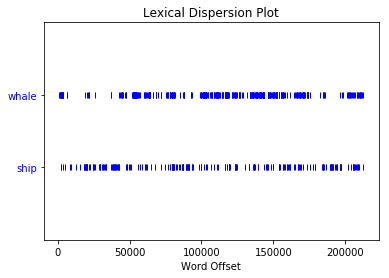
\includegraphics[height=0.6\textheight]{fig/dispersion}
\end{frame}

% move on to scikit-learn / pandas for extracting keywords with statistics
\subsection{Discovering distinctive keywords}
\begin{frame}{Distinctive words}
    Finding statistically characteristic words in a text:
    \begin{itemize}
        \item Identify important topics (content words)
        \item Identify stylistic characteristics (function words)
        \item Contrast two (sets of) texts (keyness)
    \end{itemize}

    Keyword selection methods:
    \begin{itemize}
        \item Simple word frequency
        \item Chi-square
        \item tf-idf
    \end{itemize}

    % Example applications in DH?
\end{frame}

\begin{frame}[fragile]{Why not normal frequencies?}
\begin{lstlisting}
In: moby_dick.vocab()
Out: FreqDist({'the': 13694, 'of': 6531, 'and': 5932, 'a': 4493, 'to': 4459,
    'in': 3850, 'that': 2679, 'his': 2428, 'I': 1723, 'with': 1649, ...})

In: austen_sense.vocab()
Out: FreqDist({'to': 4010, 'the': 3847, 'of': 3535, 'and': 3191, 'her': 2135,
    'a': 1996, 'in': 1833, 'was': 1773, 'I': 1673, 'she': 1257, ...})
\end{lstlisting}

\begin{itemize}
    \item The most frequent words are function words (up to, say, 50 words).
    \item Informative about style and authorship.
        \url{https://programminghistorian.org/en/lessons/introduction-to-stylometry-with-python}
    \item Mostly pretty similar and uninformative about content.
    \item Simple solution: throw away frequent ``stop words''
\end{itemize}
\end{frame}

\begin{frame}[fragile]{Chi-square: Most distinctive words across two texts}
    \begin{reference}
        %\url{http://www.thegrammarlab.com/?nor-portfolio=understanding-keyness} \\
        %\url{https://liferay.de.dariah.eu/tatom/feature_selection.html}
        \url{https://github.com/ariddell/tatom/blob/develop/source/feature_selection.rst}
    \end{reference}
% issues: uses numpy, pandas, scikit-learn
\begin{lstlisting}[style=smaller]
import numpy as np
from sklearn.feature_extraction.text import CountVectorizer
from sklearn.feature_selection import chi2
filenames = ['MELVILLE, Herman - Moby Dick.txt',
        'AUSTEN, Jane - Sense and Sensibility.txt']
vectorizer = CountVectorizer(input='filename')
document_term_matrix = vectorizer.fit_transform(filenames)
vocab = np.array(vectorizer.get_feature_names_out())
keyness, pvalues = chi2(document_term_matrix, filenames)
ranking = np.argsort(keyness)[::-1]
print(vocab[ranking][:10])
\end{lstlisting}
Result:
\begin{lstlisting}
['the', 'her', 'she', 'whale', 'of', 'and', 'in', 'elinor', 'his', 'that']
\end{lstlisting}
% the keyness scores express to what extent the assumption that the two texts have the same word frequencies is violated.
% the keyness scores do not distinguish words that are more characteristic of text A vs B.
\end{frame}

\begin{frame}[fragile]{tf-idf}
\begin{reference}\scriptsize
    %\url{https://suzil.ai/2019/01/15/extract-keywords-from-text-snippets-using-tfidf-and-sklearn/}
    \url{https://kavita-ganesan.com/python-keyword-extraction/}
    % issues: uses numpy, pandas, scikit-learn
    \url{https://programminghistorian.org/en/lessons/analyzing-documents-with-tfidf}
\end{reference}
tf-idf = term frequency / document frequency

    \begin{itemize}
        \item Intuition: words that frequently occur in few documents \\
            are most interesting.
        \item Finds good topical words: what is unique about this document?
        \item Only works if you have a large number of documents! \\
            (i.e., large corpus, say 100+ texts)
        \item Example application: automatically categorizing
            social media posts
    \end{itemize}
\end{frame}

\subsection{Named Entity Recognition}
\begin{frame}[fragile]{Named Entity Recognition (NER)}
\begin{definition}
    \structure{Named Entity Recognition} identifies names of persons,
    organizations, and locations in a text.
    An entity consists of one or more words and has a label.
\end{definition}
    Applications:
    \begin{itemize}
        \item Identify frequently mentioned characters in a text
        \item Map locations mentioned in text
        \item Explore related characters (mentioned in same paragraph)
    \end{itemize}
\pause

Install Spacy:
\begin{lstlisting}
!conda install -c conda-forge spacy
!python -m spacy download en_core_web_sm
\end{lstlisting}
\end{frame}

\begin{frame}[fragile]{Applying NER to a text}
\begin{lstlisting}
import spacy
nlp = spacy.load("en_core_web_sm")
text = """The identity of the Facebook whistleblower who ...
and that the company has tried to hide that evidence."""

doc = nlp(text)
for ent in doc.ents:
    print(ent.label_, ent.start, ent.end, ent.text)
\end{lstlisting}
\begin{verbatim}
CARDINAL 8 11 tens of thousands
DATE 29 31 recent weeks
WORK_OF_ART 36 39 60 Minutes"
TIME 39 41 Sunday night
PERSON 42 44 Frances Haugen
DATE 47 52 37-year-old
\end{verbatim}
\end{frame}

\begin{frame}{Summary}
    \begin{itemize}
        \item Searching keywords
        \item Discovering keywords
        \item Named Entity Recognition
    \end{itemize}
\end{frame}

% \begin{frame}{Mini-project}
%     \structure{Proposal}:
%     \begin{itemize}
%         \item Mini-project instead of take-home exam.
%         \item Same deadline, start now, work individually
%         \item Pick text analysis method (sentiment analysis, keyword analysis)
%         \item Pick dataset from your field (a few options will be made available)
%         \item Think of a simple (answerable) research question
%         \item \structure{Hand in}:
%             Notebook with code, quantitative results, interpretation,
%             and discussion.
%     \end{itemize}
% \end{frame}

\begin{frame}{Background reading}
    \begin{itemize}
        \item See all the links on the slides \dots (clickable)
        \item Chapter 5 Text Analysis of \url{https://melaniewalsh.github.io/Intro-Cultural-Analytics/}
    \end{itemize}
\end{frame}

\end{document}
